\documentclass[border=2pt]{standalone}
\usepackage{pgfplots}
\usepgfplotslibrary{fillbetween}
\usepackage{amsmath}
\usepackage{amssymb}
\usepackage{bm}


\def \firstmode {4}
\def \secondmode {10}

\def \p {6.2}
\def \newp {9.25}
\def \firstx {7.22}
\def \secondx {8.23}

\definecolor{darkcyan}{rgb}{0.0, 0.55, 0.55}
\definecolor{darkcerulean}{rgb}{0.03, 0.27, 0.49}

\colorlet{fcolor}{violet}
\colorlet{errcolor}{darkcyan}
\definecolor{projcolor}{named}{black}
\colorlet{dotcolor}{fcolor}
\colorlet{boundcolor}{darkcerulean}
\definecolor{newdotcolor}{named}{green}
\definecolor{arrowcolor}{named}{blue}

\pgfplotsset{ticks=none,
	domain=-1:15,
	/pgf/declare function={
		f(\x) = 3+.5*exp(-((\x-\firstmode)/2)^2) + 4*exp(-((\x-\secondmode)/2)^2) - exp(\x - 14) - 2*exp(-\x);
	},
	/pgf/declare function={
		err(\x) = 0.5+0.2*(\x-\p)^2;
	},
	/pgf/declare function={
		bound(\x) = f(\x) - err(\x) - .5;
	},
	layers/my layer set/.define layer set={
		background,
		pre main,
		main,
		foreground
	}{},
	% activate the newly created layer set
	set layers=my layer set,
}

\pgfplotsset{every axis/.style={scale only axis}}

\begin{document}
	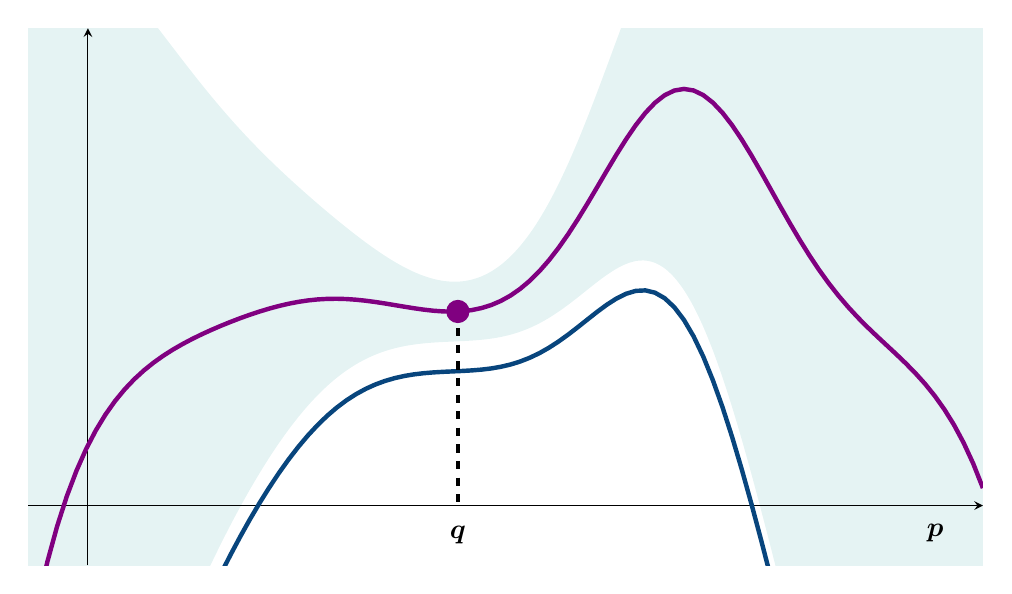
\begin{tikzpicture}
	\begin{axis}[
	height=0.5625\textwidth,
	width=\textwidth,
	xmin=-1,ymin=-1,
	xmax=15,ymax=8, 
	samples=100,
	xticklabel=\empty,
	yticklabel=\empty,
	axis lines = middle,
	xlabel=$\bm{p}$,
	%ylabel=$\bm{\mu}$,
	y label style={at={(axis description 		
			cs:.035,.9)},anchor=south},
	x label style={at={(axis description 		
			cs:.95,0.025)},anchor=south},]
	
	%True function
	\addplot[name path=perf, fcolor, ultra thick]{f(x)};
	
	%Error
	\addplot[name path=up, draw=none, forget plot, smooth]
		{f(x)+err(x)};
	\addplot[name path=low, draw=none, forget plot, smooth]
		{f(x)-err(x)};
	\addplot[errcolor, fill opacity=0.1, forget plot] fill between[of=up and low];
	
	%Current point
	\addplot[dotcolor, mark size = 4pt, only marks,samples at={\p}]{f(x)};
%	\addplot[boundcolor, mark size = 3pt, only marks,samples at={\p}]{bound(x)};
	\node[] at (axis cs: \p, -.5) {$\bm{q}$};
	
	%Lower bound
	\addplot[name path=perf, boundcolor, ultra thick]{bound(x)};

	%New point

	
	%Projections
	\addplot[dashed, projcolor, very thick, ]
		coordinates{(\p,{f(\p)}) (\p,0)};
	\end{axis}
	\end{tikzpicture}
\end{document}